\section{Experimental Setup}
\label{sec:setup}

% Figure 3 sits at the bottom of the page where the Results begin ([b], stfloats).
\begin{figure*}[b]
    \centering
    \resizebox{\linewidth}{!}{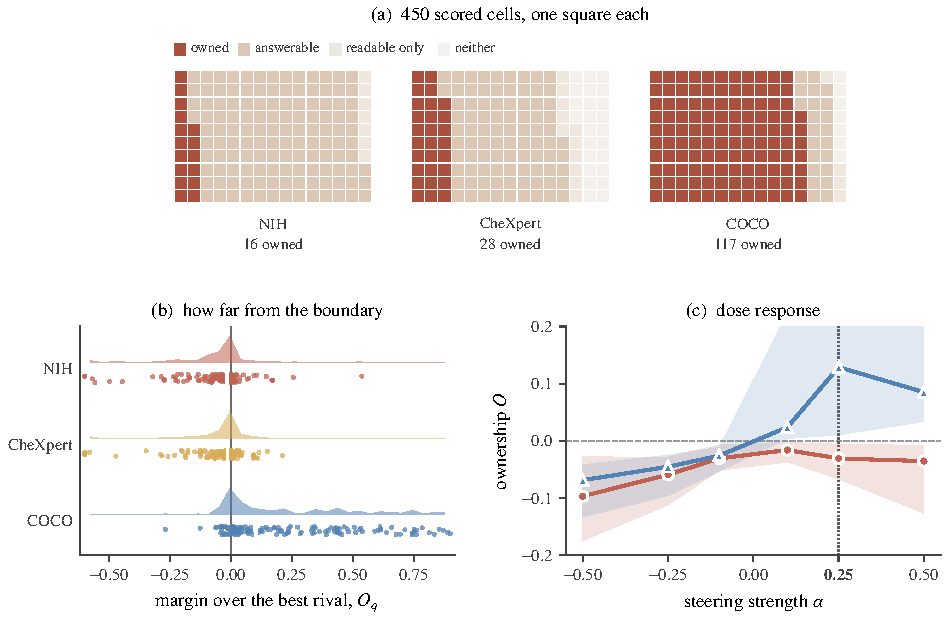
\includegraphics{figures/fig2_overview.pdf}}
    \caption{\textbf{Margins and dose response across the grid.} (a) The margin $O_q$ of each cell over its strongest competing write, as a density above and one point per cell below; the vertical line at zero is the ownership boundary and the tick is the median. (b) Median ownership and interquartile range over 25 blocks against the steering strength; the dotted line marks the graded steering strength $\alpha=+0.25$, and the COCO band is clipped at $0.2$. The share of cells passing each grade is in Figure~\ref{fig:teaser}.}
    \label{fig:overview}
\end{figure*}

\paragraph{Checkpoints.}
We evaluate \cfCheckpoints{} instruction-tuned checkpoints, 3B to 72B, from \cfFamiliesWord{} families. Six families are general-purpose: Qwen2.5-VL \citep{bai2025qwen25vl}, Qwen3-VL \citep{qwen2025qwen3vl}, InternVL3.5 \citep{wang2025internvl35}, Gemma~3 \citep{gemma2025gemma3}, LLaVA-1.5 \citep{liu2024improved}, and Llama~3.2~Vision \citep{meta2024llama32vision}. Six are medical: MedGemma \citep{sellergren2025medgemma}, Lingshu \citep{lasa2025lingshu}, LLaVA-Med \citep{li2023llavamed}, CheXagent \citep{chen2024chexagent}, HuatuoGPT-Vision \citep{chen2024huatuogptvision}, and LLaVA-Rad \citep{zambranochaves2025llavarad}. Three of them, CheXagent-2-3B, CheXagent-8B, and LLaVA-Rad-7B, have vision towers trained on chest radiographs (Table~\ref{tab:cf-models}; Appendix~\ref{app:cf-grid}).

\paragraph{Datasets and cohorts.}
NIH ChestX-ray14 \citep{wang2017chestxray} and CheXpert Plus \citep{chambon2024chexpertplus} supply frontal radiographs with report-derived labels \citep{irvin2019chexpert} for six findings each, and COCO \citep{lin2014coco} supplies six object categories as a natural-image control (Appendix~\ref{app:cf-labels}). One fixed cohort per dataset, shared by every checkpoint and disjoint across roles, holds 20{,}000 training rows for the probes and the answer direction, 400 calibration rows for the readable and answerable grades, and 600 test rows for every write (Appendix~\ref{app:repro-cohorts}).

\paragraph{Questions and scale.}
Each concept is asked as a yes/no question, with five further templates as held-out wordings (Appendix~\ref{app:protocol}). Writes use $\alpha=+0.25$, with a sweep over five further strengths. The campaign comprises \cfBlocks{} blocks, \cfCells{} scored concept cells, about 30 million scored answers, and roughly 3{,}000 A100-hours (Appendix~\ref{app:cf-coverage}).

\paragraph{Measures.}
A model \emph{answers best} on a cell when its clean-answer AUROC is at least \cfStratTopEdge{}. The \emph{own-question share} is the fraction of the positive answer change, $\max(W_{q,d},0)$ averaged over checkpoints, that falls on the written concept's own question. Reader differences are measured in \emph{refit standard deviations} of $O_q$ across the three probe fits, and an \emph{effect floor} of $0.05$ on $W_{q,q}$ and $O_q$ sets a minimum effect size.
